\documentclass{egpubl}
\usepackage{eg2017}

\ShortPresentation      % uncomment for (final) Short Conference Presentation

\electronicVersion % can be used both for the printed and electronic version

\ifpdf \usepackage[pdftex]{graphicx} \pdfcompresslevel=9
\else \usepackage[dvips]{graphicx} \fi

\PrintedOrElectronic

% prepare for electronic version of your document
\usepackage{t1enc,dfadobe}

\usepackage{egweblnk}
\usepackage{cite}

%%% Added packages and commands %%%
\usepackage[usenames,dvipsnames]{xcolor}
\usepackage{amsmath}
\usepackage{amssymb}
\usepackage{hyperref}

\newcommand{\added}[1]{{\color{Red}\textbf{#1}}} % do not need this probably
\newcommand{\note}[3]{{\color{#2}\textbf{#1: #3}}}
\newcommand{\henrik}[1]{\note{HENRIK}{WildStrawberry}{#1}}
\newcommand{\john}[1]{\note{JohnKa}{RubineRed}{#1}}
\newcommand{\IGNORE}[1]{}
\graphicspath{{fig/}}

% correct bad hyphenation here
\hyphenation{to-po-lo-gi-cal-ly to-po-lo-gy      ini-tial  col-our pat-ches}

\title[Non-rectangular gradient mesh tool]
	{A Gradient Mesh Tool for Non-Rectangular Gradients}

% for anonymous conference submission please enter your SUBMISSION ID
% instead of the author's name (and leave the affiliation blank) !!
\author[short1007]
{\parbox{\textwidth}{\centering short1007}
        \\
% School/Institution here (if accepted)
	{\parbox{\textwidth}{\centering } }
}

% if the Editors-in-Chief have given you the data, you may uncomment
% the following five lines and insert it here
%
% \volume{27}   % the volume in which the issue will be published;
% \issue{1}     % the issue number of the publication
% \pStartPage{1}      % set starting page

\begin{document}

% \teaser{
%  \includegraphics[width=\linewidth]{eg_new}
%  \centering
%   \caption{New EG Logo}
% \label{fig:teaser}
% }

\maketitle

\begin{abstract}
The gradient mesh tool, implemented in vector graphics software like Adobe Illustrator, is a much-used tool for creating and manipulating complex colour gradients. The mesh-based tool is restricted to rectangular control meshes, making it hard for the user to work with more complicated shapes such as shapes with holes. We propose a new gradient mesh tool that supports non-rectangular control meshes, with native support for a wide range of different shapes. Additionally, our tool supports flexible mesh and colour editing functionality that makes local edits easier than with previous tools. A user study indicates that our tool is easier to use in the setting of drawing colour gradients inside complicated shapes with holes.

\begin{classification} % according to http:http://www.acm.org/about/class/1998
\CCScat{Computer Graphics}{I.3.4}{Graphics Utilities}{Paint systems}
\end{classification}

\end{abstract}

\section{Introduction}
\label{sec:intro}

In vector graphics design, working with complex colour functions is challenging. The restrictions of the linear gradient tool is one reason designers turn to pixel-based tools, like Adobe Photoshop, when the design turns complicated. In the past decade, this issue has been acknowledged in the research community and a wide range of different approaches have been proposed to make the design of colour gradients more effortless \cite{Orzan:2008,Lopez-Moreno:2013}.

In this paper, we propose a new tool for gradient mesh editing. The gradient mesh tool, found in vector graphics packages like Adobe Illustrator and Corel CorelDraw, is a much-used tool for complex colour gradient design. It is especially useful in scenarios where the easier-to-use linear gradient tool does not suffice. However, it does not support non-rectangular gradients: the control mesh that the user directly creates and edit must be of rectangular topology. Using a recently proposed interpolation technique for gradient meshes of arbitrary topology~\cite{Lieng:2016}, we propose a tool where the user can create and manipulate non-rectangular colour gradients, like the one shown in Fig.[REF-teaser].

Mesh-based colour gradient design is similar to 3D mesh editing: the user is presented with a net of control points that can be manipulated to influence the underlying manifold. In vector graphics, the user is restricted to the 2D canvas and objects are only drawn from a single perspective, reducing the number of degrees of freedom to the user compared to 3D modelling. Current tools are further restricted to rectangular topologies, making the interactive tools only applicable to the rectangular setting. This is demonstrated in Section~\ref{sec:RW}, where it is demonstrated that current rectangular-restricted interaction techniques cannot be easily extended to the non-rectangular setting. In Sections~\ref{sec:method} and \ref{sec:DP}, we propose a set of new tools to accommodate editing of gradient meshes of arbitrary topology. Our new tool is compared against Adobe Illustrator's gradient mesh tool in a user study (Section~\ref{sec:evaluation}), which indicates that our tool is preferable for designing non-rectangular gradients.

In summary, our primary contribution is a new, publicly-available, tool for gradient mesh design. It is the only gradient mesh tool that natively supports gradients of non-rectangular topology and compared with a state-of-the-art gradient mesh tool, our user study indicates that our contribution simplifies the process of working with non-rectangular gradients.

\section{Related work}
\label{sec:RW}

There have been proposed a myriad of techniques and tools for colouring, shading, and texturing of 2D graphics (e.g. \cite{Vergne:2012, Shao:2012}). Such techniques often employ underlying primitives and technology, like vector graphics gradients or the graphics pipeline, to achieve high-level tools for various creation and editing operations. On the other hand, the gradient mesh tool is a general tool for the creation and manipulation of complex colour gradients. Although there are techniques that employ gradient meshes for high-level operations, like 2D material editing~\cite{Lopez-Moreno:2013}, these techniques also enforce additional assumptions to fit their specific application.

There are three major vector primitives for defining colour gradients: linear gradients, gradient meshes, and diffusion curves~\cite{Orzan:2008}. In this paper, we do not argue against or for any of these well established primitives. We instead envision a range of vector graphics tools that build upon these primitives to offer the best possible software suite for both professional and novice designers.

The gradient mesh tool is mostly relevant to our work. The tool is available in all of the three major vector graphics suites (Adobe Illustrator, Corel CorelDraw, and Inkscape). All of these tools employ similar interpolation techniques, variants of Ferguson or Bezier patches (although the specific implementation is not publicly available in other than Inkscape which employs Coons patches conforming to the current SVG 2 specification). Thus, all previous tools are restricted to gradients of rectangular topology, as shown in Fig.~\ref{fig:IllustratorVsOur} (using Illustrator's tool as an example). Our approach takes advantage of a recent gradient mesh interpolation technique that supports arbitrary mesh topology~\cite{Lieng:2016}. Being able to model non-rectangular gradient meshes provides significant practical advantages, especially for vector shapes with holes.

Looking at the three software packages, it is Adobe Illustrator that provides the most comprehensive gradient mesh tool, with an elegant point-and-click interface to add control points to the mesh. We have therefore only compared our tool to this state-of-the-art tool. This comparison is outlined in Section~\ref{sec:evaluation}.

\begin{figure}
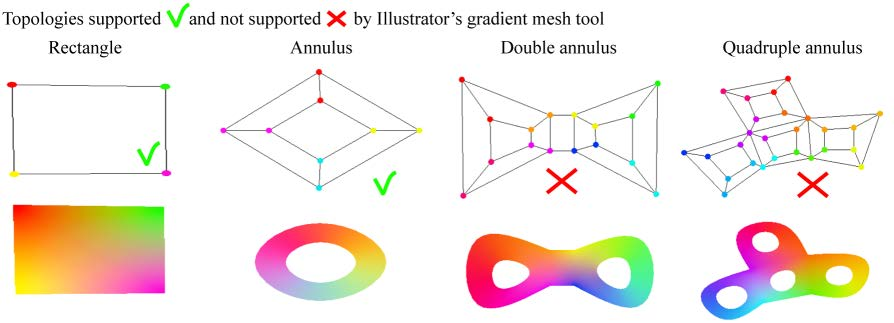
\includegraphics[]{illustratorVsOur.jpg}
\caption{\john{Should we use a new image, or is it OK to refer to the article and alter some of the original caption?}}
\label{fig:IllustratorVsOur}
\end{figure}

\section{Problem description}
\label{sec:overview}

In this section, we outline the interaction techniques available in previous gradient mesh tools (with reference to Adobe's tool) and describe why these techniques cannot easily be extended to the setting of non-rectangular control meshes.

The gradient mesh tool offers two approaches to mesh creation. The first option converts a vector graphics object compatible with rectangular gradients (i.e. a vector shape without any holes) to a grid of control points. This option requires the user to input the number of rows and columns of the to-be created gradient mesh. The second option is a point-and-click interface where the user clicks on a location inside the target shape and a new row and column is created at the clicked location (Fig.~\ref{fig:illustratorCreateMesh}).

The first option is incompatible with non-rectangular gradient meshes. This is because the creation is dependent on a grid representation of the mesh, as the user has provided a given number of rows and columns. However, a non-rectangular mesh cannot be represented by a grid-like data structure. An arbitrary non-rectangular mesh corresponds to general polygonal meshes and can be represented by data structures such as the half-edge data structure.

The second option is attractive for couple of reasons. First, the creation operation is independent from the underlying data structure: a single click on the canvas can give rise to several interpretations and the effect of the click can be separated from the representation of the underlying data (for example, via data abstraction). Second, one can easily imagine such an interaction to be intuitive. From a user perspective, a click inside a vector shape with a gradient tool can indicate that a given colour should influence the region of the click.

On the other hand, the point-and-click interface introduces several challenges. Already in the regular setting, there are challenging shapes that require ad-hoc solutions, as shown in Fig.~\ref{fig:adHocPentagon}. \john{Is it correct image?} Additionally, the interaction produces a global mesh alteration: when a control point is added, a new row and column is added to the entire mesh. It is therefore challenging to achieve local gradient edits and the user must consequently plan the structure of the mesh prior to editing so that the number of rows and columns is kept to a minimum. In the non-rectangular setting, it is even more challenging. Fig.~\ref{fig:adHocPentagon} illustrates a user click inside a polygon adjacent to a pentagon. The effect of such an interaction is ambiguous and many results could be imagined. The two solutions outlined in the figure introduces either a T-junction or a high-valence control point. Both options produce a mesh that is of poorer quality compared to the original mesh.

In conclusion, the user interaction already supported by the gradient mesh tool is hard to extend to the more flexible setting of non-rectangular control meshes. The representation of the mesh, using a polygonal mesh representation, does not support the simple addition of rows and columns as one can do with grid-based meshes. In the next section, we outline a different approach to interaction that we hypothesise is more feasible in the non-rectangular setting compared with the two approaches described above.

\begin{figure}[t]
	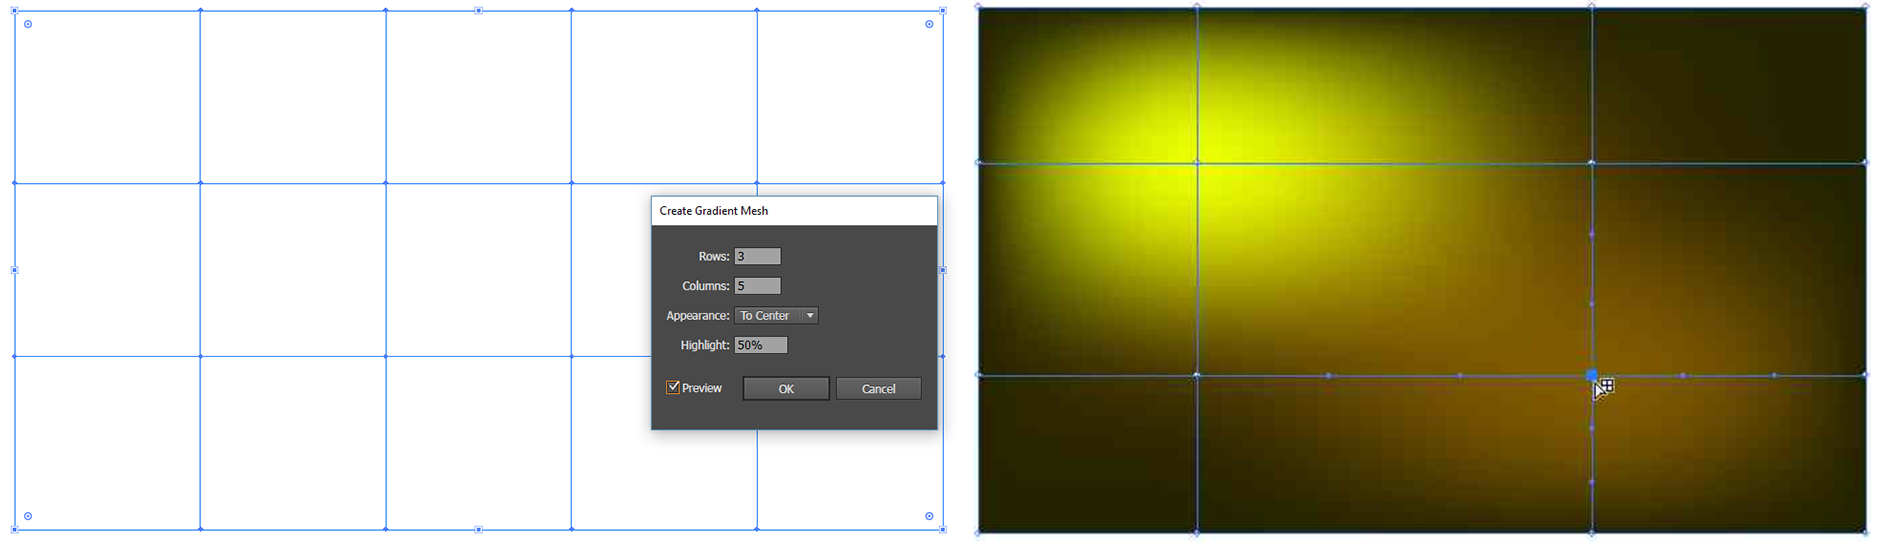
\includegraphics[width=0.5\textwidth]{IllustratorCreateGradientMeshCombined.png}
	\caption{In Adobe Illustrator you have two options when creating a gradient mesh. Either via an input box (left), or via  point-and click operations (right).}
	\label{fig:illustratorCreateMesh}
\end{figure}

\begin{figure}[t]
	\centering
	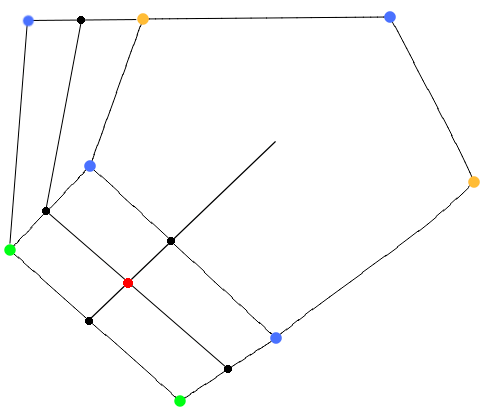
\includegraphics[height=0.25\textheight]{pentagonMesh.png}
	\caption{The red point indicates the location of were the user clicked. A new point is made at this location. As mentioned in Section~\ref{sec:overview}, a new column and row is added to the entire mesh. It is introduced new vertices at each edge intersection (the black points). The issue occurs when we add a new vertex in a polygon adjacent to a pentagon. If the pentagon are split following the red dashed line we will suddenly introduce several new vertices as the line will propagate to adjacent polygons. One could alternatively introduce new vertices on the edges were no polygon is adjacent, but the solution is indeed ad-hoc either way. }
	\label{fig:adHocPentagon}
\end{figure}

\section{Tools for creating non-rectangular gradient meshes}
\label{sec:method}

Our approach is inspired by tools found in 3D polygonal modelling. Specifically, we take inspiration from the pen tool in SketchUp, which is a tool for drawing polygonal meshes in 3D. Building on such a basic tool for creating polygonal meshes in 2D, we provide tools for operations such as face deletion, and edge split and collapse.

We envision the user to create initial meshes \textit{face-by-face}, which can later be refined and manipulated by operations like edge split and merge. Our \textbf{line tool} enables the user to create a single polygonal face. The user starts by creating a single face. The mesh is then expanded by iteratively adding faces to it. To add a face, the user selects an existing mesh vertex. After the edges of the face have been placed on the canvas, the user close the face by clicking on an existing vertex (which must already be connected to a face), including the initial vertex. This allows for a non-manifold mesh, as shown in Fig. REF. \john{Burde kanskje skrive noe om du legger til face inni et face(?):} If the face to add is internal -- that is, inside an existing face -- the closing vertex must be an other than the initial vertex. This is due to the implementation of creating internal faces (subject to change).

The user can further locally edit and refine the control mesh. The \textbf{edge split tool} splits a selected edge into two pieces. The inserted control point should then be connected to another mesh point to avoid valence-2 control points. Note that edges are modelled as cubic Bezier curves: each control point is associated with a gradient constraint for each of its edges that control the local influence of the colour of the control point. Such gradient constraints is a standard feature of gradient meshes. To ensure that the curve of the edge is maintained when the edge is split, the position of the new control point is calculated using De Casteljau's algorithm. Finally, adjacent edges can be collapsed for mesh simplification and faces can be removed to introduce holes (Fig. REF).

\begin{figure*}[t]
	\centering
	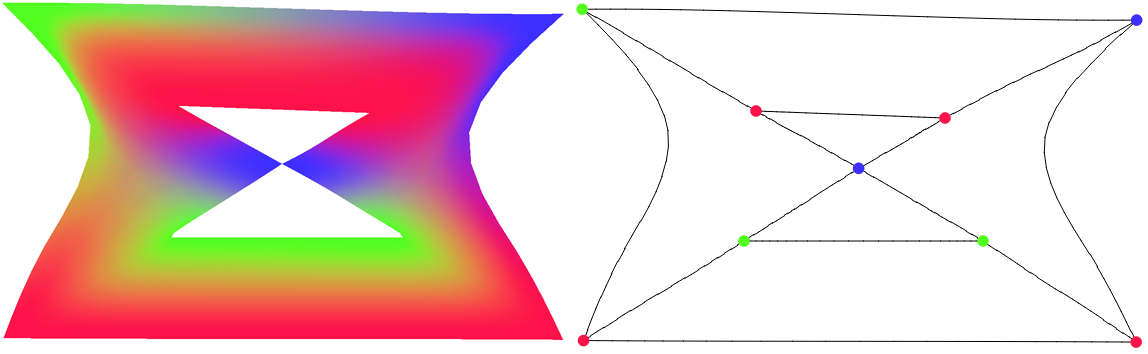
\includegraphics[height=0.25\textheight]{HoleAndNonManifoldMesh.png}
	\caption{ }
	\label{fig:adHocPentagon}
\end{figure*}

\section{Multi-resolution editing with colour points}
\label{sec:DP}

Creating and editing a sparse mesh will suffice for many scenarios, especially when the colour function does not change much. However, the user might want more detailed control in certain areas. One option is to subdivide the mesh to a level that captures the necessary level of detail. This approach is both time consuming for the user and unnecessarily complicates the mesh. As previously mentioned, we employ the method of Lieng et al.~\cite{Lieng:2016} as the underlying interpolation technique. This method employs subdivision surfaces and supports the feature of multi-resolution mesh manipulation; that is, mesh alteration on different level of detail. 

We employ this multi-resolution feature to associate colour points to mesh faces. If the user wants a specific colour influencing the colour function inside the face, colour points are added to the face. This is similar to the point-and-click interface described in Section~\ref{sec:overview}. Instead of directly altering the mesh, the clicked position is added to the face data as a colour point. This colour point is stored with a colour value and mean-value (barycentric) coordinates~\cite{Floater:2003} with respect to the face control points. Barycentric coordinates are used so that when the face is moved, its colour points are moved correspondingly.

When producing the colour gradient, the colour points are used to influence the subdivision procedure a selected number of subdivision iterations... \henrik{add fancy stuff here...}

\section{Results}
\label{sec:results}

Our tool was implemented in C++ with use of the libraries Qt (\url{https://www.qt.io/}) for the GUI and OpenMesh (\url{http://www.openmesh.org/}) for easy mesh manipulation with the half-edge data structure. The implementation consists of 3 -- three -- layers. Qt stands for the graphical representation and listen for changes on the mesh. OpenMesh represents the middle layer, that parses changes from the GUI to the internal layer. The internal layer handle mesh subdivision, interpolation, and rendering, by employing the method presented by Lieng et al.~\cite{Lieng:2016}, as mentioned in Section~\ref{sec:intro}.

\henrik{resultater: referer til video. Beskriv hvordan hull opprettes.}
\john{Det nevnes vel hvordan hull lages i Sec~\ref{sec:method} ?}

\section{Informal user study}
\label{sec:evaluation}

Our gradient mesh tool were tested by 5 subjects -- 2 professionals designers and 3 art students --- who all had experience with Adobe Illustrator. The subjects were given an introduction to our program and to the relevant tools in Illustrator. They were given two task; the first task was to make a rectangular gradient mesh. The second task was to make a gradient mesh with two holes. The subjects were not allowed to use layering, that is, none of the meshes should overlap. The tests were complemented with an user survey, which 4 of 5 test subjects answered. Images they could take inspiration from, results, and time consumption is shown in Fig. REF . 

One test subject answered the following in the user survey: \textit{"[...] I enjoyed the experience from the tested tool more than Illustrator when it came to the tasks given. Both were difficult for a beginner, but at least the tested tool made more sense: especially with deleting frames to create holes."}. Some of the subjects got tired, and somewhat angry, of doing test 2 in Illustrator that they conclude the test before they were finished or happy with the result. Additional data and videos from the user study can be found in the supplementary article. 

\henrik{beskriv user study og resultater, med et diagram som viser tider? Referer til `supplementary material' (ekstra dokument med samme latex template). All informasjon går i supplementary material dokument.}

\section{Future work}
\label{sec:FW}

Though our gradient mesh tool offers opportunities to work with non-rectangular gradient meshes, it is not an full experience graphical design software application. Future work will be to rewrite our tool as a plug-in for the Adobe Illustrator. This presents several issues, as the underlying mesh representation in Illustrator differs from ours. Still, one approach can be to take use of Pixar's OpenSubdiv library (\url{http://graphics.pixar.com/opensubdiv/}) and integrating this with Illustrators SDK.

\henrik{future work (nok med to ting): lage en illustrator plugin. Burde bruke et ekstern subdivision bibliotek, som Pixar's OpenSubdiv, og må integrere det med illustrator sitt bibliotek.}

\section{Conclusion}

We have introduced a new tool for working with non-rectangular gradient meshes. In contrast to gradient mesh tools in other applications -- like Adobe Illustrator -- our tool allows for quick and easy creation and alternation of gradient meshes which can be of arbitrary topology and contain holes. Users are given more detailed control over the resulting mesh than with previous tools, as they can employ use of colour points and multi resolution editing of the mesh.

\john{write more}

\bibliographystyle{eg-alpha}

\bibliography{refs}

\end{document}